\documentclass{article}
\usepackage{hyperref}
\usepackage{amsmath}
\usepackage{graphicx} % Required for inserting images
\usepackage{subcaption} %  for subfigures environments
\usepackage{float}

\title{Path tracer}
\author{Javier Sancho Olano \\ \href{mailto:815520@unizar.es}{815520@unizar.es}}
\date{Junio 2024}

\begin{document}

\maketitle

\tableofcontents
\newpage

\section{Introducción}
La ecuación de render es una ecuación integral que describe la cantidad de
radiancia emitida de un punto \(\mathbf{x}\) de una superficie hacia una
dirección \(\mathbf{\omega_{o}}\)

\begin{equation}
  L_o(\mathbf{x}, \mathbf{\omega_{o}}) = L_e(\mathbf{x}, \mathbf{\omega_{o}}) + \int_{\Omega} L_i(\mathbf{x}, \mathbf{\omega_{i}}) \cdot f_r(\mathbf{x}, \mathbf{\omega_{i}}, \mathbf{\omega_{o}}) \cdot  |\mathbf{n} \cdot \mathbf{\omega_{i}}| \, d\omega_{i}
\end{equation}

\begin{figure}[h]
  \centering 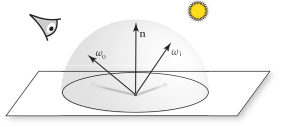
\includegraphics[width=0.6\textwidth]{imgs/rendereq.png}
  \caption{Ilustración del problema de la ecuación de render}
\end{figure}

donde:
\begin{itemize}
  \item \(\mathbf{x}\) es un punto en el espacio
  \item \(\mathbf{\omega_{o}}\) es la dirección de salida
  \item \(\mathbf{n}\) es la normal de la superficie
  \item \(\mathbf{\omega_{i}}\) es la dirección de la radiancia incidente
  \item \(L_o(\mathbf{x}, \mathbf{\omega_{o}})\) es la cantidad de radiancia
        emitida de un punto \(\mathbf{x}\) de una superficie hacia una dirección
        \(\mathbf{\omega_{o}}\)
  \item \(L_e(\mathbf{x}, \mathbf{\omega_{o}})\) es la radiancia que la
        superficie emite en el punto \(\mathbf{x}\), hacia
        \(\mathbf{\omega_{o}}\)
  \item \(\int_{\Omega} ... \, d\omega_{i}\) es una integral sobre la hemiesfera
        \(\Omega\)
  \item \(L_i(\mathbf{x}, \mathbf{\omega_{i}}) \) es la radiancia incidente en
        \(\mathbf{x}\) desde la dirección \(\mathbf{\omega_{i}}\)
  \item \(f_r(\mathbf{x}, \mathbf{\omega_{i}}, \mathbf{\omega_{o}}) \) es la
        BTDF, la proporción de radiancia reflejada hacia \(\mathbf{\omega_{o}}\)
        desde \(\mathbf{\omega_{i}}\) en el punto \(\mathbf{x}\)
  \item \(|\mathbf{n} \cdot \mathbf{\omega_{i}}|\) a.k.a \(\cos\theta_{i}\) es
        el factor que ajusta la contribución de la radiancia incidente respecto
        a \(\mathbf{\omega_{i}}\)
\end{itemize}

Entonces \textit{path tracer} hace referencia a la técnica que se usará para
resolver esta ecuación. El algoritmo \textit{path tracer} usará el estimador de
Monte Carlo para aproximar la integral de render.

Si quisiéramos evaluar una integral como esta \(\int^{b}_{a} f(x) \; dx\), y
dado una variable aleatoria uniforme \(X_{i} \in [a, b]\), el estimador de Monte
Carlo dice que la esperanza del siguiente estimador, \(E[F_{N}]\) es igual a la
integral.
\[F_{N}=\frac{b-a}{N} \sum_{i=1}^{N} f(X_{i}) \]
\[E[F_{N}]= \int^{b}_{a} f(x) \; dx\]

Si la variable aleatoria \(X_{i}\) se extrae de una PDF arbitraria entonces la
esperanza del siguiente estimador sigue siendo la integral.
\begin{equation}
  F_{N}=\frac{1}{N} \sum_{i=1}^{N} \frac{f(X_{i})}{p(X_{i})}
\end{equation}
\begin{equation}
  E[F_{N}]= \int^{b}_{a} f(x) dx
\end{equation}

Aplicando la ecuación 2 a nuestra ecuación de render (Eq. 1):

\begin{equation}
  L_o(\mathbf{x}, \mathbf{\omega_{o}}) \approx L_e(\mathbf{x}, \mathbf{\omega_{o}}) + \frac{1}{N} \sum_{i=1}^{N} \frac{L_i(\mathbf{x}, \mathbf{\omega_{i}}) \cdot f_r(\mathbf{x}, \mathbf{\omega_{i}}, \mathbf{\omega_{o}}) \cdot  |\mathbf{n} \cdot \mathbf{\omega_{i}}|}{p(\omega_{i})}
\end{equation}

Para un camino (\(N=1\))
\(\{\mathbf{x_{1}}, \mathbf{x_{2}}, ..., \mathbf{x_{k}}\}\),
\(L_{i}(\mathbf{x_{j}}, \mathbf{\omega_{o}})=L_{o}(\mathbf{x_{j+1}}, \mathbf{\omega_{o}})\)
y cuando la superficie emita, simplificaremos:
\(L_{o}(\mathbf{x}, \mathbf{\omega_{o}})=L_{e}(\mathbf{x}, \mathbf{\omega_{o}})\)

Podemos descomponer la radiancia incidente en dos componentes:
\[L_i(\mathbf{x}, \mathbf{\omega_{i}}) = L_{i,d}(\mathbf{x}, \mathbf{\omega_{i}}) + L_{i,i}(\mathbf{x}, \mathbf{\omega_{i}}),\]

\begin{itemize}
  \item \(L_{i,d}(\mathbf{x}, \mathbf{\omega_{i}})\) es la radiancia directa que
        llega a \(\mathbf{x}\) desde una fuente de luz
  \item \(L_{i,i}(\mathbf{x}, \mathbf{\omega_{i}})\) es la radiancia indirecta
        que llega a \(\mathbf{x}\) tras haber sido reflejada o refractada.
\end{itemize}

Por lo que la ecuación de render se puede reescribir como:

\begin{equation}
  \begin{split}
    L_o(\mathbf{x}, \mathbf{\omega_{o}}) & = L_e(\mathbf{x}, \mathbf{\omega_{o}}) + \int_{\Omega} (L_{i,d}(\mathbf{x}, \mathbf{\omega_{i}}) + L_{i,i}(\mathbf{x}, \mathbf{\omega_{i}})) \cdot f_r(\mathbf{x}, \mathbf{\omega_{i}}, \mathbf{\omega_{o}}) \cdot  |\mathbf{n} \cdot \mathbf{\omega_{i}}| \, d\omega_{i} \\
                                         & = L_e(\mathbf{x}, \mathbf{\omega_{o}})
                                           + \int_{\Omega} L_{i,d}(\mathbf{x}, \mathbf{\omega_{i}}) \cdot f_r(\mathbf{x}, \mathbf{\omega_{i}}, \mathbf{\omega_{o}}) \cdot  |\mathbf{n} \cdot \mathbf{\omega_{i}}| \, d\omega_{i} \\
                                         &\quad\quad\quad\quad\quad\  + \int_{\Omega} L_{i,i}(\mathbf{x}, \mathbf{\omega_{i}}) \cdot f_r(\mathbf{x}, \mathbf{\omega_{i}}, \mathbf{\omega_{o}}) \cdot  |\mathbf{n} \cdot \mathbf{\omega_{i}}| \, d\omega_{i} \\
  \end{split}
\end{equation}

De esta forma podemos extender la ecuación 4 y estimar la radiancia directa para
luces puntuales:

\begin{equation}
  \begin{split}
    L_o(\mathbf{x}, \mathbf{\omega_{o}}) & = L_e(\mathbf{x}, \mathbf{\omega_{o}}) + \frac{L_{i,i}(\mathbf{x}, \mathbf{\omega_{i}}) \cdot f_r(\mathbf{x}, \mathbf{\omega_{i}}, \mathbf{\omega_{o}}) \cdot  |\mathbf{n} \cdot \mathbf{\omega_{i}}|}{p(\omega_{i})} \\
                                         & + \sum_{p \in luces} \frac{L_{i,d}(\mathbf{x}, \mathbf{\omega_{p}}) \cdot f_r(\mathbf{x}, \mathbf{\omega_{p}}, \mathbf{\omega_{o}}) \cdot  |\mathbf{n} \cdot \mathbf{\omega_{p}}|}{p(\omega_{p})}
  \end{split}
\end{equation}

Y como la PDF de \(\omega_{p}\) siempre sera 1, la ecuación se simplifica a:
\begin{equation}
  \begin{split}
    L_o(\mathbf{x}, \mathbf{\omega_{o}}) & = L_e(\mathbf{x}, \mathbf{\omega_{o}}) + \frac{L_{i,i}(\mathbf{x}, \mathbf{\omega_{i}}) \cdot f_r(\mathbf{x}, \mathbf{\omega_{i}}, \mathbf{\omega_{o}}) \cdot  |\mathbf{n} \cdot \mathbf{\omega_{i}}|}{p(\omega_{i})} \\
                                         & + \sum_{p \in luces} L_{i,d}(\mathbf{x}, \mathbf{\omega_{p}}) \cdot f_r(\mathbf{x}, \mathbf{\omega_{p}}, \mathbf{\omega_{o}}) \cdot  |\mathbf{n} \cdot \mathbf{\omega_{p}}|
  \end{split}
\end{equation}

Finalmente aplicaremos el estimador de Monte Carlo (Eq. 3) para aproximar la
integral de render y la radiancia de un pixel \(L\) será la media de todos los
caminos que pasan por el pixel:
\begin{equation}
  L \approx \frac{1}{spp} \sum_{i=1}^{spp} L_{o}(\mathbf{x_{1i}}, \mathbf{\omega_{o1i}})
\end{equation}

\section{Implementación del integrador}
Cuando un rayo intersecta con un objeto en la escena, se calculará la
información del choque (\(\mathbf{x}, \mathbf{\omega_{o}}, \mathbf{n}\),
material), que se usará para calcular \(L_o(\mathbf{x}, \mathbf{\omega_{o}})\) o
\(L_{i,i}(\mathbf{x}, \mathbf{\omega_{i}}) \).

Para ello necesitamos implementar todos los términos que aparecen en la ecuación
7:

\begin{itemize}
  \item \(L_e(\mathbf{x}, \mathbf{\omega_{o}})\) es devuelto por el la instancia
        del material y en nuestra implementación es constante para todo
        \(\mathbf{x}\) y \(\mathbf{\omega_{o}}\)
  \item \(f_r(\mathbf{x}, \mathbf{\omega_{i}}, \mathbf{\omega_{o}}) \) es
        devuelto por la instancia del material, representa una BTDF, por lo que
        puede ser una BRDF difusa, una BRDF especular o una BTDF refracta. Cuando
        se llama a esta función, además de devolver el valor de la BSDF, pone en
        \(\omega_{i}\) la siguiente dirección del camino. Si la BRDF es difusa,
        \(\omega_{i}\) se puede muestrear con la distribución del ángulo sólido
        o con la del coseno. Por otro lado si la BRDF es delta, \(\omega_{i}\)
        no se muestrea y se calcula deterministicamente.

        Cabe destacar que esta función en el código se llama \textit{sampleFr}
        ya que ``\textit{samplea}'' \(\omega_{i}\) y es diferente de \textit{Fr}
        no ``\textit{samplea}'' \(\omega_{i}\).
  \item \(p(\mathbf{\omega_{i}})\) es acorde al muestreo de la BRDF difusa
        seleccionado y es 1 en caso de ser BSDF delta.
  \item \(|\mathbf{n} \cdot \mathbf{\omega_{i}}|\) a.k.a \(\cos\theta_{i}\) es
        el factor que ajusta la contribución de la radiancia incidente respecto
        a \(\mathbf{\omega_{i}}\)
  \item \(L_{i,d}(\mathbf{x}, \mathbf{\omega_{i}})\) es la radiancia directa que
        llega a \(\mathbf{x}\) desde una fuente de luz, se calcula como la
        potencia de la luz dividida por la distancia al cuadrado.
\end{itemize}

\section{Convergencia}

Para estudiar la convergencia del \textit{path tracer} vamos a renderizar la
escena \textit{Cornell Box} con distintos samples per pixel. Adicionalmente y
para ilustrar la importancia de que \(p\) siga \(|\mathbf{n}\cdot \omega_{i}|\),
se mostrará una comparación de las dos distribuciones implementadas para
muestrear \(\Omega\). Figuras 2-6.

\subsection{Samples per pixel}

El \textit{path tracer}, usando \textit{n spp} converge al resultado correcto de
la integral de forma \(\frac{1}{\sqrt{n}}\) (Si asumimos que esos \textit{n}
samples son independientes y \(\sigma\) es la desviación estándar de la
distribución, el valor medio calculado para el pixel, \(\bar{x}\), tendrá
asociado un error estándar, \(\sigma_{\bar{x}}=\frac{\sigma}{\sqrt{n}}\)). Es
decir, cuadruplicando \textit{n} se reduce el error a la mitad o en otras
palabras, cuadruplicando \textit{n} mejora la imagen el doble.

En mi opinión, este hecho se puede observar muy bien en las Figuras 2-6. En las
cuales se puede ver como la calidad de la imagen se duplica al cuadruplicar los
samples per pixel.

\begin{figure}
\begin{subfigure}[h]{0.4\linewidth}
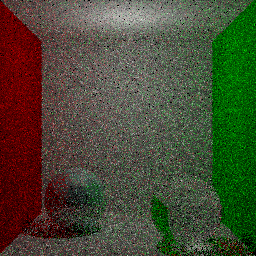
\includegraphics[width=\linewidth]{imgs/cosine_box2.png}
\caption{Uniform cosine sampling}
\end{subfigure}
\hfill
\begin{subfigure}[h]{0.4\linewidth}
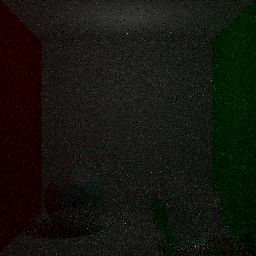
\includegraphics[width=\linewidth]{imgs/solid_angle_box2.png}
\caption{Uniform solid angle sampling}
\end{subfigure}%
\caption{Cornell Box con 2 samples per pixel}
\end{figure}

\begin{figure}
\begin{subfigure}[h]{0.4\linewidth}
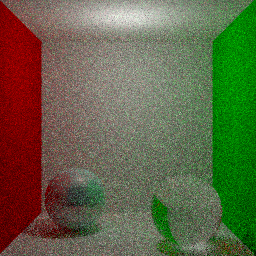
\includegraphics[width=\linewidth]{imgs/cosine_box8.png}
\caption{Uniform cosine sampling}
\end{subfigure}
\hfill
\begin{subfigure}[h]{0.4\linewidth}
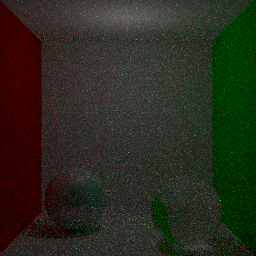
\includegraphics[width=\linewidth]{imgs/solid_angle_box8.png}
\caption{Uniform solid angle sampling}
\end{subfigure}%
\caption{Cornell Box con 8 samples per pixel}
\end{figure}

\begin{figure}
\begin{subfigure}[h]{0.4\linewidth}
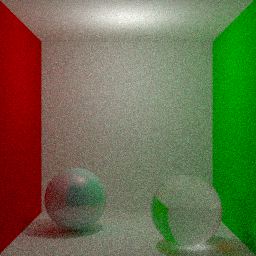
\includegraphics[width=\linewidth]{imgs/cosine_box32.png}
\caption{Uniform cosine sampling}
\end{subfigure}
\hfill
\begin{subfigure}[h]{0.4\linewidth}
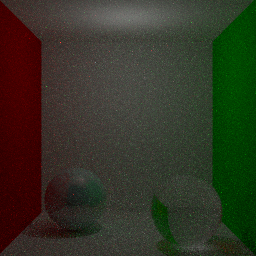
\includegraphics[width=\linewidth]{imgs/solid_angle_box32.png}
\caption{Uniform solid angle sampling}
\end{subfigure}%
\caption{Cornell Box con 32 samples per pixel}
\end{figure}

\begin{figure}
\begin{subfigure}[h]{0.4\linewidth}
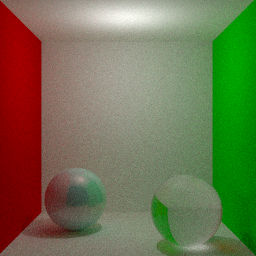
\includegraphics[width=\linewidth]{imgs/cosine_box128.png}
\caption{Uniform cosine sampling}
\end{subfigure}
\hfill
\begin{subfigure}[h]{0.4\linewidth}
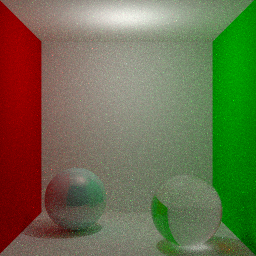
\includegraphics[width=\linewidth]{imgs/solid_angle_box128.png}
\caption{Uniform solid angle sampling}
\end{subfigure}%
\caption{Cornell Box con 128 samples per pixel}
\end{figure}

\begin{figure}
\begin{subfigure}[h]{0.4\linewidth}
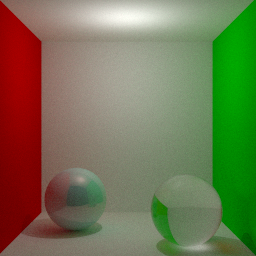
\includegraphics[width=\linewidth]{imgs/cosine_box512.png}
\caption{Uniform cosine sampling}
\end{subfigure}
\hfill
\begin{subfigure}[h]{0.4\linewidth}
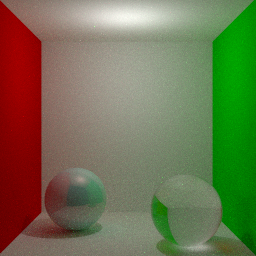
\includegraphics[width=\linewidth]{imgs/solid_angle_box512.png}
\caption{Uniform solid angle sampling}
\end{subfigure}%
\caption{Cornell Box con 512 samples per pixel}
\end{figure}

\subsection{Influencia de los materiales sobre la convergencia}

Los materiales con BRDF difusa convergen más rápido que aquellos con BRDFs
delta. En primer lugar, los materiales difusos podrán aprovechar el
\textit{next-level estimation} para calcular la contribución de las luces
puntuales en ese punto. Además el muestreo del siguiente \(\mathbf{\omega_{i}}\)
en la hemiesfera favorece la convergencia frente a un muestreo de
\(\mathbf{\omega_{i}}\) determinista.

\subsection{Fuentes de luz}
Las escenas con luces puntuales convergen significativamente más rápido que
aquellas con luces de área como se puede ver en Figuras 7-11. Este hecho se
explica dado que las luces puntuales usan \textit{next-event estimation}, que
muestrean directamente la luz de las fuentes puntuales en cada camino. En
contraste, en el caso de las luces en área, se necesitarán más caminos para que
alguno de ellos pueda explorar la dirección de la luz de área, lo que ralentiza
la convergencia.

\begin{figure}[H]
\begin{subfigure}[h]{0.4\linewidth}
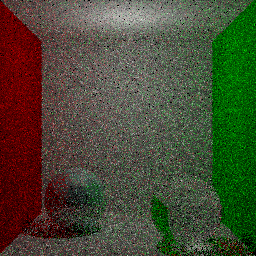
\includegraphics[width=\linewidth]{imgs/cosine_box2.png}
\caption{Luz puntual}
\end{subfigure}
\hfill
\begin{subfigure}[h]{0.4\linewidth}
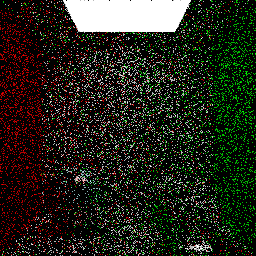
\includegraphics[width=\linewidth]{imgs/area_box2.png}
\caption{Luz de área}
\end{subfigure}%
\caption{Cornell Box con 2 samples per pixel}
\end{figure}

\begin{figure}[H]
\begin{subfigure}[h]{0.4\linewidth}
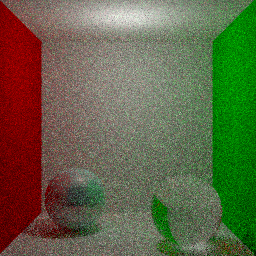
\includegraphics[width=\linewidth]{imgs/cosine_box8.png}
\caption{Luz puntual}
\end{subfigure}
\hfill
\begin{subfigure}[h]{0.4\linewidth}
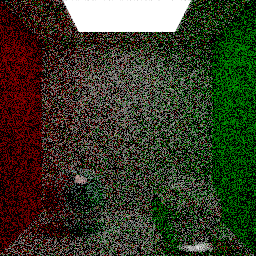
\includegraphics[width=\linewidth]{imgs/area_box8.png}
\caption{Luz de área}
\end{subfigure}%
\caption{Cornell Box con 8 samples per pixel}
\end{figure}

\begin{figure}[H]
\begin{subfigure}[h]{0.4\linewidth}
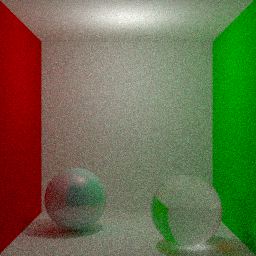
\includegraphics[width=\linewidth]{imgs/cosine_box32.png}
\caption{Luz puntual}
\end{subfigure}
\hfill
\begin{subfigure}[h]{0.4\linewidth}
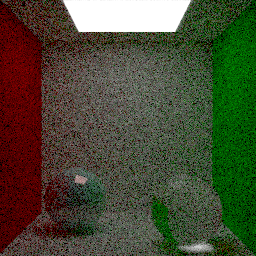
\includegraphics[width=\linewidth]{imgs/area_box32.png}
\caption{Luz de área}
\end{subfigure}%
\caption{Cornell Box con 32 samples per pixel}
\end{figure}

\begin{figure}[H]
\begin{subfigure}[h]{0.4\linewidth}
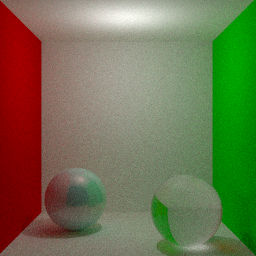
\includegraphics[width=\linewidth]{imgs/cosine_box128.png}
\caption{Luz puntual}
\end{subfigure}
\hfill
\begin{subfigure}[h]{0.4\linewidth}
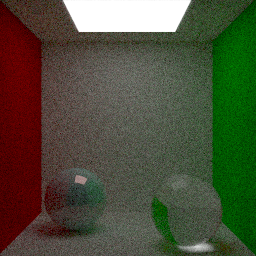
\includegraphics[width=\linewidth]{imgs/area_box128.png}
\caption{Luz de área}
\end{subfigure}%
\caption{Cornell Box con 128 samples per pixel}
\end{figure}

\begin{figure}[H]
\begin{subfigure}[h]{0.4\linewidth}
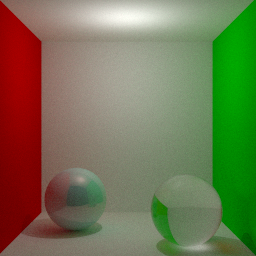
\includegraphics[width=\linewidth]{imgs/cosine_box512.png}
\caption{Luz puntual}
\end{subfigure}
\hfill
\begin{subfigure}[h]{0.4\linewidth}
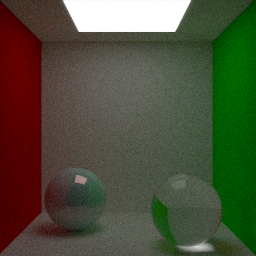
\includegraphics[width=\linewidth]{imgs/area_box512.png}
\caption{Luz de área}
\end{subfigure}%
\caption{Cornell Box con 512 samples per pixel}
\end{figure}

\newpage

\section{Iluminación global}

El algoritmo \textit{path tracer} es capaz de simular todos los cuatro efectos
de la iluminación global: \textit{hard shadows}, \textit{soft shadows},
\textit{color bleeding} y \textit{causics}. \\

Las \textbf{\textit{hard shadows}} son muy fácil de obtener con el algoritmo
\textit{path tracer}, y ya hemos visto cómo lucen en las Figuras 2-6, basta con
añadir a la escena luces puntuales. \\

Las \textbf{\textit{soft shadows}} son muy fáciles de obtener también. Figuras
7-11, y basta con añadir a la escena alguna luz de área. \\

\begin{figure}[H]
\begin{subfigure}[h]{0.4\linewidth}
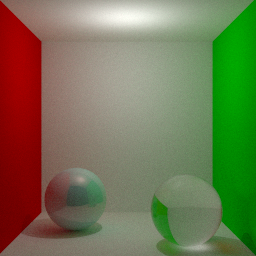
\includegraphics[width=\linewidth]{imgs/hard.png}
\caption{Hard shadow}
\end{subfigure}
\hfill
\begin{subfigure}[h]{0.4\linewidth}
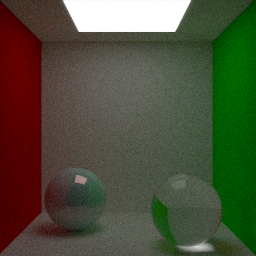
\includegraphics[width=\linewidth]{imgs/soft.png}
\caption{Soft shadow}
\end{subfigure}
\caption{Comparativa de sombras}
\end{figure}

\textbf{\textit{Color bleeding}} es el fenómeno por el cual una superficie es
coloreada por el color reflejado de otra superficie cercana. También es muy
fácil de conseguir, basta con colocar dos objetos cerca uno del otro. Se puede
ver en las paredes de la caja de las Figuras 2-11 o con más claridad en la
Figura 13 tanto en la pared de atrás, en el suelo, en la cara o en la espalda
del conejo de plástico. \\

\begin{figure}[H]
\centering
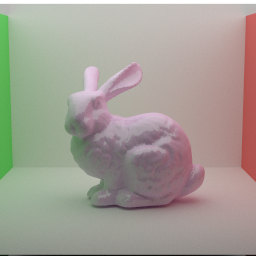
\includegraphics[width=0.6\linewidth]{imgs/plastic_bunny.png}
\caption{Conejo de plástico}
\end{figure}

Finalmente las \textbf{\textit{cáusticas}} son algo más difícil de conseguir ya
que al tratarse de rayos de luz muy concentrados en un punto, es poco probable
que el algoritmo genere estos caminos eficientemente. Sin embargo con un gran
número de \textit{samples per pixel}, la geometría y la iluminación correcta se
puede conseguir: TODO CAMBIAR imagen
\begin{figure}[H]
\centering
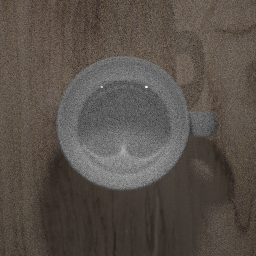
\includegraphics[width=0.6\linewidth]{imgs/nephroid.png}
\caption{Taza de cerámica (difusa + especular) (medio metida en una mesa) en la
  que se puede ver una cáustica nefroide}
\end{figure}

\section{Extensiones}
\subsection{Triángulos}
Además de las esferas, se ha implementado el triángulo. Para ello he seguido mas
o menos la estructura de datos propuesta por el libro
\href{https://www.pbr-book.org/3ed-2018/Shapes/Triangle_Meshes}{pbrt}\footnote{https://www.pbr-book.org/3ed-2018/}
para almacenar mayas de triangulos eficientemente.

En resumen, una representación natural sería almacenar cada triángulo con las
posiciones de sus tres vértices, sin embargo, una representación más eficiente
en memoria sería almacenar la maya de triángulos con un array de posiciones,
donde cada triangulo solo almacena los 3 índices de los vértices en el array de
posiciones. Además se almacena un array de normales por vértice y un array de
coordenadas de textura por vértice.

La implementación de la intersección ray-triangle fue sorprendentemente sencilla
gracias al gran artículo en Wikipedia y se basa en el algorimo de
\href{https://en.wikipedia.org/wiki/M%C3%B6ller%E2%80%93Trumbore_intersection_algorithm}{Möller-Trumbore}.

\subsubsection{Modelos 3D}
El siguiente paso tras implementar los triángulos es cargar modelos 3D en
formato \textit{.ply}. Para ello he implementado mi propia mini-librería para
cargar archivos \textit{.ply}.

Vamos a ver algunas imágenes con modelos 3D de triángulos. Figura 15.

\begin{figure}[H]
\begin{subfigure}[h]{0.4\linewidth}
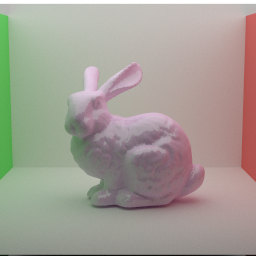
\includegraphics[width=\linewidth]{imgs/plastic_bunny.png}
\caption{Stanford bunny de plástico}
\end{subfigure}
\hfill
\begin{subfigure}[h]{0.4\linewidth}
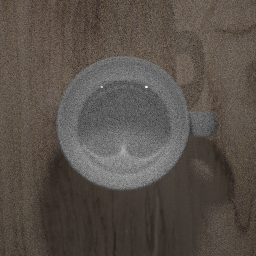
\includegraphics[width=\linewidth]{imgs/nephroid.png}
\caption{Cáustica en una taza de café}
\end{subfigure}

\begin{subfigure}[h]{0.4\linewidth}
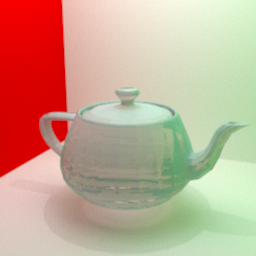
\includegraphics[width=\linewidth]{imgs/crystal_teapot.png}
\caption{Utah teapot de cristal}
\end{subfigure}
\hfill
\begin{subfigure}[h]{0.4\linewidth}
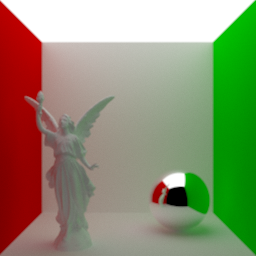
\includegraphics[width=\linewidth]{imgs/lucy.png}
\caption{Lucy en Cornell Box}
\end{subfigure}
\caption{Algunos modelos con triángulos}
\end{figure}

\subsection{Texturas}
Las texturas son una generalización de los materiales. En lugar de devolver un
coeficiente constante, devuelven un coeficiente que depende de la posición del
punto de intersección. Por lo que es posible aplicar texturas diferentes para
coeficientes difusos, especulares y refractantes.

La implementación gira en torno a la interfaz \texttt{Texture}. De esta forma,
he podido implementar texturas de color sólido, texturas de imagen y texturas
procedurales.

\subsubsection{Environment maps}

Con las texturas ya implementadas, he añadido los \textit{environment maps}.
Estos \textit{environment maps} simulan un entorno alrededor de las escenas
calculando la posición en la textura esférica cuando un rayo no intersecta con
la escena.

\begin{figure}[H]
\begin{subfigure}[h]{0.4\linewidth}
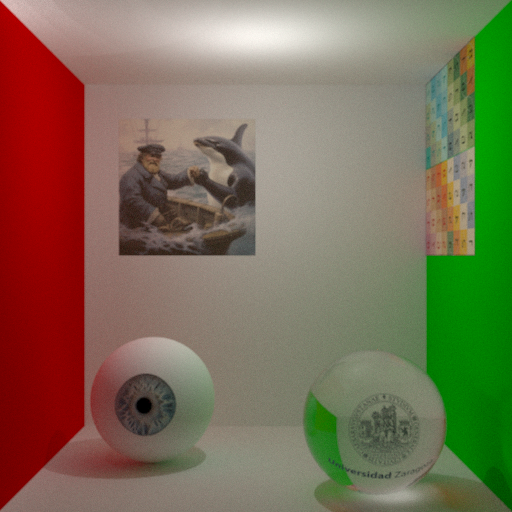
\includegraphics[width=\linewidth]{imgs/corneltex.png}
\caption{Texturas en triángulos, esferas y mexcla de materiales con texturas}
\end{subfigure}
\hfill
\begin{subfigure}[h]{0.4\linewidth}
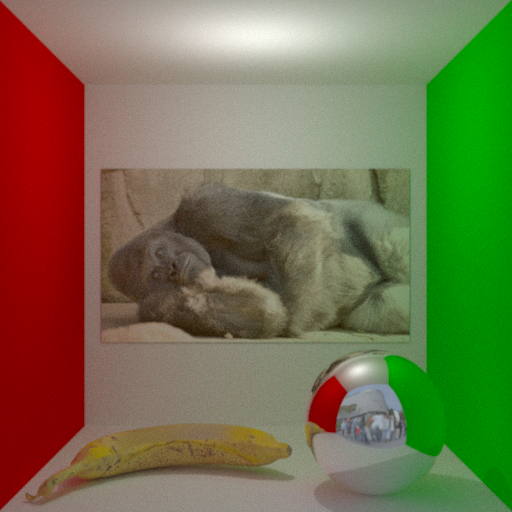
\includegraphics[width=\linewidth]{imgs/harambe.png}
\caption{Modelos 3D con texturas y environment map}
\end{subfigure}
\caption{Algunos ejemplos de texturas}
\end{figure}

\subsubsection{Texturas procedurales}
TODO

\subsection{Multi-threading}
Esto realmente cuesta considerarlo como una extensión pues gracias a OpenMP, con
simplemente añadir \texttt{\#pragma omp parallel for} antes de un bucle for,
este automáticamente te lo paraleliza. OpenMP viene incluido con el compilador
(GCC 4.2 o nuevas y Clang/LLVM 3.7 o nuevas).

Si usar esto no está permitido en la asignatura, basta con eliminar
\texttt{-fopenmp} de las flags de compilación y el nuevo ejecutable funcionará
pero sin multithreading. \\

Todas las pruebas están hechas en un Intel(R) Core(TM) i7-10750H @ 2.60GHz turbo
5.0GHz con 1.5 MiB de L2 cache y 12 MiB de L3 cache y con soporte para AVX2.

\subsubsection{Mejoras en el tiempo de renderizado}

Para analizar la mejora en el tiempo de renderizado con el multithreading, he
renderizado la escena \textit{Cornell Box (256x256)} con distintos \textit{samples per
  pixel} y he comparado el tiempo de renderizado con y sin multithreading:

\begin{center}
\begin{tabular}{||c c c||}
 \hline
 Samples per pixel & Multi thread tiempo (s) & Single thread tiempo (s) \\ [0.5ex]
 \hline\hline
 2 & 2.2427 & 1.1333 \\
 \hline
 8 & 2.2656 & 2.2783 \\
 \hline
 32 & 3.2779 & 9.9038 \\
 \hline
 128 & 10.1068 & 34.3494 \\
 \hline
 512 & 43.4335 & 146.2601 \\ [1ex]
 \hline
\end{tabular}
\end{center}

Como se puede observar, el multithreading mejora dramáticamente el tiempo de
renderizado en casi todos los casos. Sin embargo, observamos que en casos con un
número muy bajo de \textit{samples per pixel} el multithreading puede ser
contraproducente. Esto se debe a que el tiempo de crear los threads y
sincronizarlos es mayor que el tiempo de renderizado.

\subsection{BVH}
Para acelerar el renderizado de las escenas, decidí implementar \textit{Bounding
  Volume Hierarchy} (BVH). La idea es que en lugar de hacer intersecciones con
todos los objetos de la escena, construir un árbol que divida el espacio en
cajas y que cada caja contenga un número pequeño de objetos. De esta forma,
cuando un rayo intersecte con una caja, solo se harán intersecciones con los
objetos que contiene.

Mi implementación se basa en gran medida en la de
\href{https://www.pbr-book.org/3ed-2018/Primitives_and_Intersection_Acceleration/Bounding_Volume_Hierarchies}{pbrt}\footnote{https://www.pbr-book.org/3ed-2018},
y por simplicidad, el metodo de separar se limita a dividir el conjunto en dos
subconjuntos de igual tamaño recursivamente.

\subsubsection{Mejoras en el tiempo de renderizado}

Para analizar la mejora en el tiempo de renderizado con el BVH, he renderizado
la escena del \textit{Stanford Bunny (256x256)} con distintos \textit{samples
  per pixel} y he comparado el tiempo de renderizado con y sin BVH. He escogido
la escena del \textit{Stanford Bunny} ya que la escena de la \textit{Cornell
  Box} es muy pequeña y no se aprecia la mejora del BVH. Además, los test se
ralizaran con un solo thread.

TODO TODO TODO TODO 

\begin{center}
\begin{tabular}{||c c c||}
 \hline
 Samples per pixel & tiempo (s) & tiempo w/BVH (s) \\ [0.5ex]
 \hline\hline
 2 & 0 & 0 \\
 \hline
 8 & 0 & 0 \\
 \hline
 32 & 0 & 0 \\
 \hline
 128 & 0 & 0 \\
 \hline
 512 & 0 & 0 \\ [1ex]
 \hline
\end{tabular}
\end{center}

\subsection{Visualizador en tiempo real}
Desde que comienzo la asignatura me llamó mucho la atención la idea de conseguir hacer un visualizador en tiempo real de los algoritmos visto en clase. En mis tiempos libres he estado probando diferentes métodos como implementar un \textit{path tracer} en un shader de GLSL o usar CUDA, pero todo esto significaba empezar de cero y no sabía muy bien como integrarlo a este trabajo.

Hasta que no hace mucho descubri \href{https://www.raylib.com/}{Raylib}\footnote{https://www.raylib.com/}, una libreria en C para hacer videojuegos y me encanto desde el primer momento por su simplicidad.

Para conseguir un visualizador en tiempo real, simplemente ejecuto unas cuantas iteraciones del path tracer, aplicó un tone-mapper y muevo la información de mi buffer a una textura de Raylib.

Para hacer más rico el visualizador, he añadido dos modos, uno en el que solo sirve como visualizador donde puedes hacer zoom y pan en la imagen Y el segundo donde puedes mover la cámara con el teclado y el ratón como un FPS.

TODO IMAGEN FPS

\subsubsection{WebAssembly}
Raylib permite compilar para practicamente cualquier plataforma por lo que me sentí gravemente tentado a compilarlo en WebAssembly y subirlo a \href{https://1sanch0.github.io/ver/}{GitHub Pages}\footnote{https://1sanch0.github.io/ver/}.

\subsection{Camaras}

La implementación de las cámaras se basa en una clase abstracta \texttt{Camera} 
el metodo \texttt{getRay}. De esta forma, es posible implementar cualquier tipo
de cámara simplemente heredando de \texttt{Camera} y sobreescribiendo el metodo
\texttt{getRay}.

Ademas, la clase \texttt{Camera} implementa los metodos \texttt{writeColor}, \texttt{writeDepth} y \texttt{writeNormal} para poder guardar la informacion del color, la profundidad y la normal de la escena respectivamente.

TODO: IMAGENES DEPTH Y NORMAL

\subsubsection{Perspective camera}
TODO (pereza)

\subsubsection{Orthographic camera}
TODO (pereza)

\subsection{Merger}
TODO (creo que lo tengo mal programado incluso xdd)

\subsection{Tone-mappers}
TODO (pereza)

\subsection{Argument Parser}
Para hacer más fácil la ejecución del programa, he implementado un \textit{argument
parser} basado en la libreria de python
\href{https://docs.python.org/3/library/argparse.html}{argparse}\footnote{https://docs.python.org/3/library/argparse.html}.

Mi implementación tiene una API muy similar y es muy fácil de usar.

TODO IMAGEN --HELP

\subsection{Barra de progreso}
Para facilitar el seguimiento de los tiempos de renderizado he implementado una
barra de progreso basada en la libreria de python
\href{https://tqdm.github.io/}{tqdm}\footnote{https://tqdm.github.io/}.

Mi implementación carace de muchas de las funcionalidades de la original pero es
suficiente para mi proposito.

TODO API E IMAGEN

\end{document}
